% !TEX root = ../MasterThesis_goto_v1.tex

%%%%%%%%%%%%%%%%%%%%%%%%%%%%%%%%%%%%%%%%%%%%%%%%%%%%%%%%%%%%%%%%%%%%%%%%%%%%%%%%%%%%%%%%%%%%%%%%%%%%%
\chapter{序論} \label{chap:Introduction}

本章では, まず\ref{Intro:StandardModel}節で素粒子の振る舞いを記述する理論である, 標準模型 (the Standard Model, SM) について紹介する。

次に\ref{Intro:InternationalLinearColliderProject}節にて, この標準模型を超える物理 (Physics beyond the Standard Model, BSM) を探索するための国際リニアコライダー (International Linear Collider, ILC) 計画についての説明を行う。
ILCが目指す物理について\ref{Intro:PhysicsofILC}節で述べ, ILCで使用する予定の検出器やソフトウェアに関する説明を\ref{Intro:InternationalLargeDetector}節と\ref{Intro:SoftwareandEventReconstructionofILC}節で行う。

更に本研究の目的について\ref{Intro:Purpose}節で, 本論文の流れについて\ref{Intro:Flow}節でそれぞれ述べ本論文の序論とする。

本章の作成にあたり, 参考文献\cite{GlobalProject, InterimDesignReport}を使用した。


%%%%%%%%%%%%%%%%%%%%%%%%%%%%%%%%%%%%%%%%%%%%%%%%%%%%%%%%%%%%%%%%%%%%%%%%%%%%%%%%%%%%%%%%%%%%%%%%%%%%%
\section{標準模型} \label{Intro:StandardModel}

宇宙の誕生や, 生物の発生と同様に, 物質の起源は人類の根元的な問いの一つである。
そのような物質を構成する最小の粒子のことを素粒子といい, その素粒子の振る舞いを記述する理論の一つが標準模型である。
標準模型によると, 素粒子はスピン半整数のフェルミ粒子とスピン整数のボース粒子に分類される。\\

標準模型ではフェルミ粒子は全てスピン$1/2$の粒子で構成され, 陽子や中性子などのハドロンを構成するクォークと電子やニュートリノなどのレプトンに分けられる。
更に, クォークは電荷が$+2/3$のアップクォーク系列と$-1/3$のダウンクォーク系列に, レプトンは電荷が$-1$の荷電レプトンと中性電荷の中性レプトン (ニュートリノ) に分けられる。
また, それぞれ世代と呼ばれるものを構成し現在は3つの世代が確認されている。
クォークの場合はアップクォーク$\textit u$, チャームクォーク$\textit c$, トップクォーク$\textit t$, ダウンクォーク$\textit d$, ストレンジクォーク$\textit s$, ボトムクォーク$\textit b$が存在する。
レプトンの場合は荷電レプトンとして, 電子$\textit e^-$, ミュー粒子$\it \mu^-$, タウ粒子$\it \tau^-$, 中性レプトンとして, 電子ニュートリノ$\it \nu_e$, ミューニュートリノ$\it \nu_{\mu}$, タウニュートリノ$\it \nu_{\tau}$が存在している。
これらの系列や世代間の違いをフレーバーと呼んでいる。

ボース粒子は基本的な四つの相互作用である, 強い相互作用, 弱い相互作用, 電磁相互作用, 重力相互作用の内, 重力相互作用を除いた三つの相互作用をそれぞれ媒介するスピン$1$のゲージ粒子と, 対称性を破り素粒子に質量を与えるスピン$0$, 中性電荷のヒッグス粒子$\it H$で構成される。
電磁相互作用を媒介する粒子として, 中性電荷の光子$\it \gamma$, 強い相互作用を媒介する粒子として, 中性電荷のグルーオン$\it g$, 弱い相互作用を媒介する粒子として, 電荷$\pm 1$のWボソン ($\it W^{\pm}$), 中性電荷のZボソン ($\it Z$) が存在する。\\

更に素粒子には, 質量やスピンが等しく電荷の正負のみが反転した反粒子が存在する。\footnote{狭義にはDirac方程式の負のエネルギー解の解釈である。}
これら反粒子と通常の粒子が衝突すると対消滅が起こり, その質量が全てエネルギーへと変換される。
一方, ある粒子の質量の二倍以上のエネルギーを生じさせた場合は対生成が起こり, その粒子と反粒子の対が生成されることがある。

以上の素粒子を標準模型の素粒子といい, 一般に図\ref{1SMParticle}のように纏められている。

\begin{figure}[htbp]
 \centering
 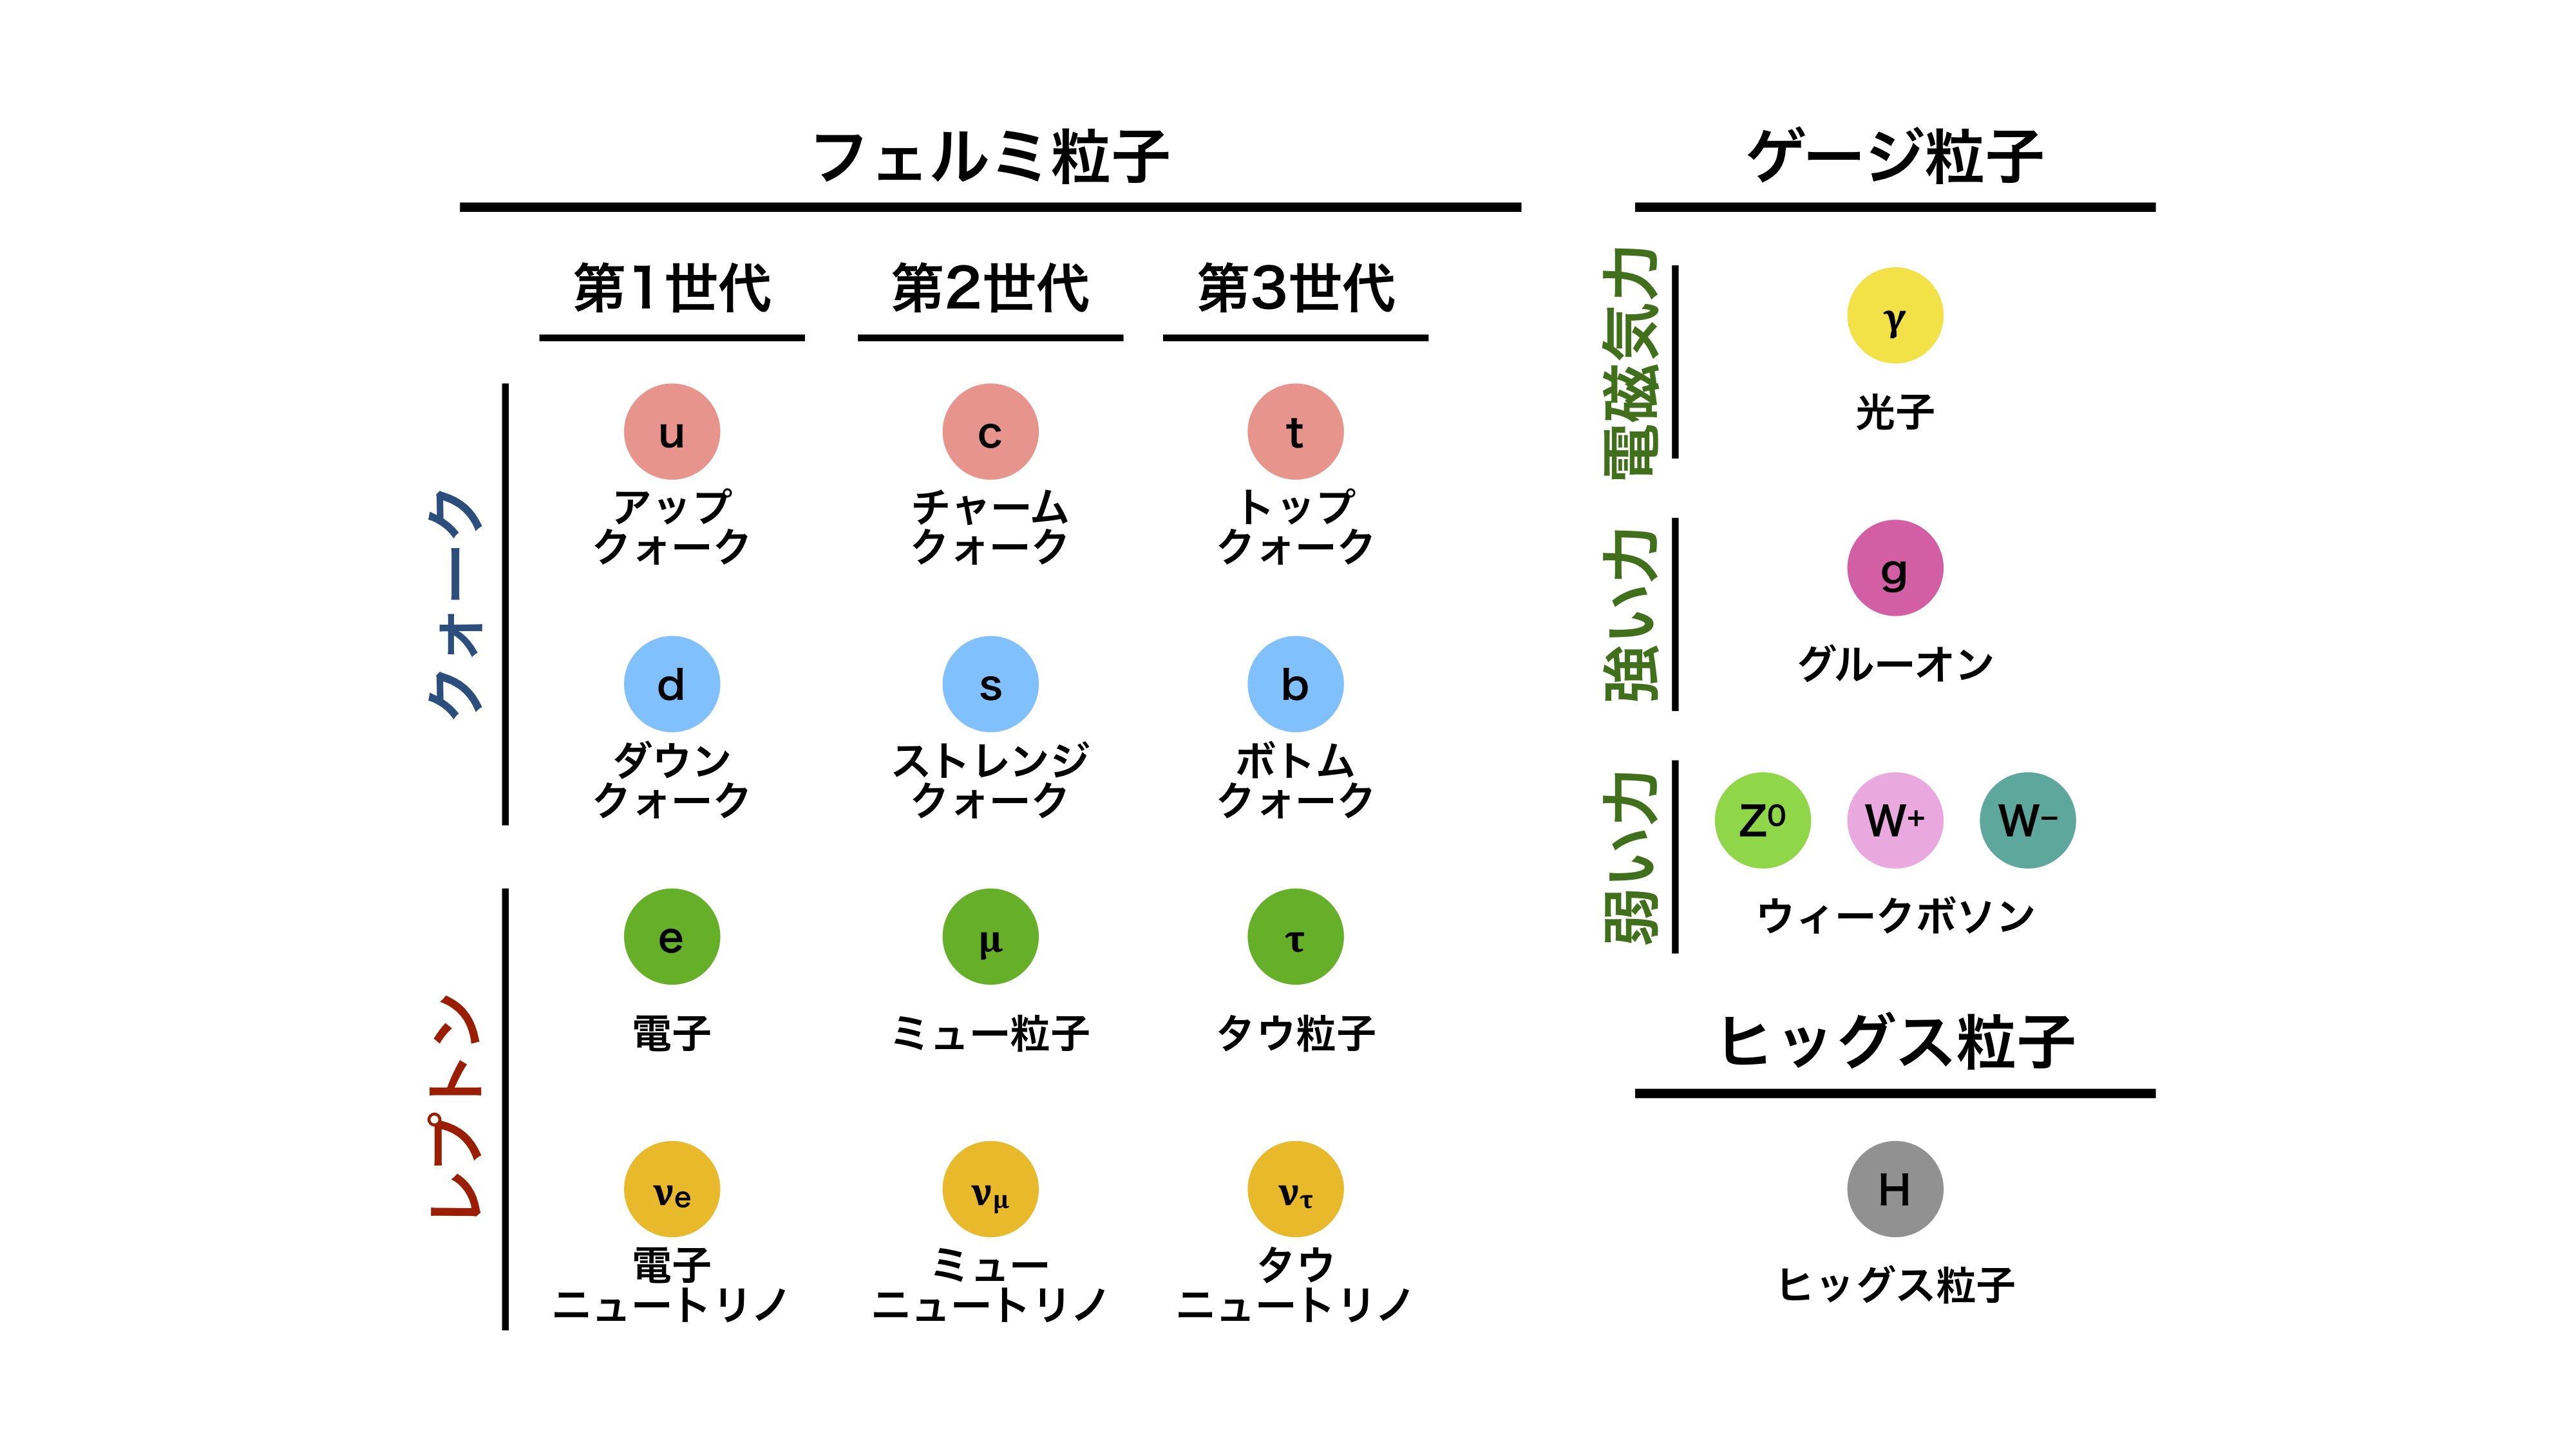
\includegraphics[width=0.9\textwidth]{Figure/1Introduction/1SMParticle.png}
 \caption{標準模型の素粒子}
 \label{1SMParticle}
\end{figure}

標準模型は様々な実験で非常によく確かめられているが, ダークマターをはじめとする幾つかの物理現象を説明できていない。
これらの標準模型で説明できない物理現象をPhysics beyond the Standard Model (BSM) といい, 現在は様々な実験施設でBSMの探索が行われている。
次節のILC計画はそのような試みの一つである。


%%%%%%%%%%%%%%%%%%%%%%%%%%%%%%%%%%%%%%%%%%%%%%%%%%%%%%%%%%%%%%%%%%%%%%%%%%%%%%%%%%%%%%%%%%%%%%%%%%%%%
\section{ILC計画} \label{Intro:InternationalLinearColliderProject}

ILC計画とは, 日本の東北にある北上山地に全長$20.5\ \mathrm{km}$の国際リニアコライダー (ILC) を建設する計画である (図\ref{2InternationalLinearCollider})。
ILC計画は国際共同研究であり, 2013年に出版されたThe Technical Design Report (TDR) \cite{ILCTDRVES} には2400人の研究者, 48ヶ国, 392の大学と研究機関のグループが署名している。

また技術開発は国際将来加速器委員会 (The International Committee for Future Accelerator, ICFA) の下, 国際推進チーム (International Development Team, IDT) によって実行されており, このIDTを2022年を目処にILC準備研究所 (ILC Pre-Lab) に移行する計画となっている。
ILC計画の今後の大まかな流れを図\ref{3ILCProject}に示す。

\begin{figure}[htbp]
 \centering
  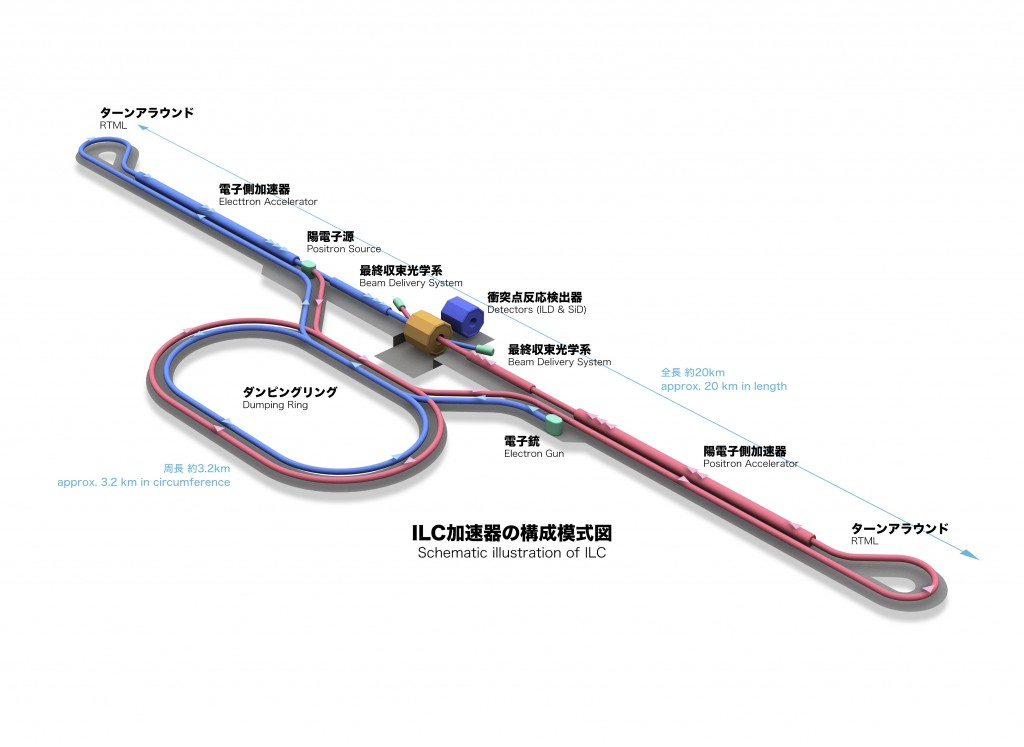
\includegraphics[trim = 0 100 0 100, width=0.9\textwidth, clip]{Figure/1Introduction/2InternationalLinearCollider.jpg}
  \caption[ILCの全体像]
                 {ILCの全体像\cite{ILCPHOTO}}
  \label{2InternationalLinearCollider}
\end{figure}

\begin{figure}[htbp]
 \centering
 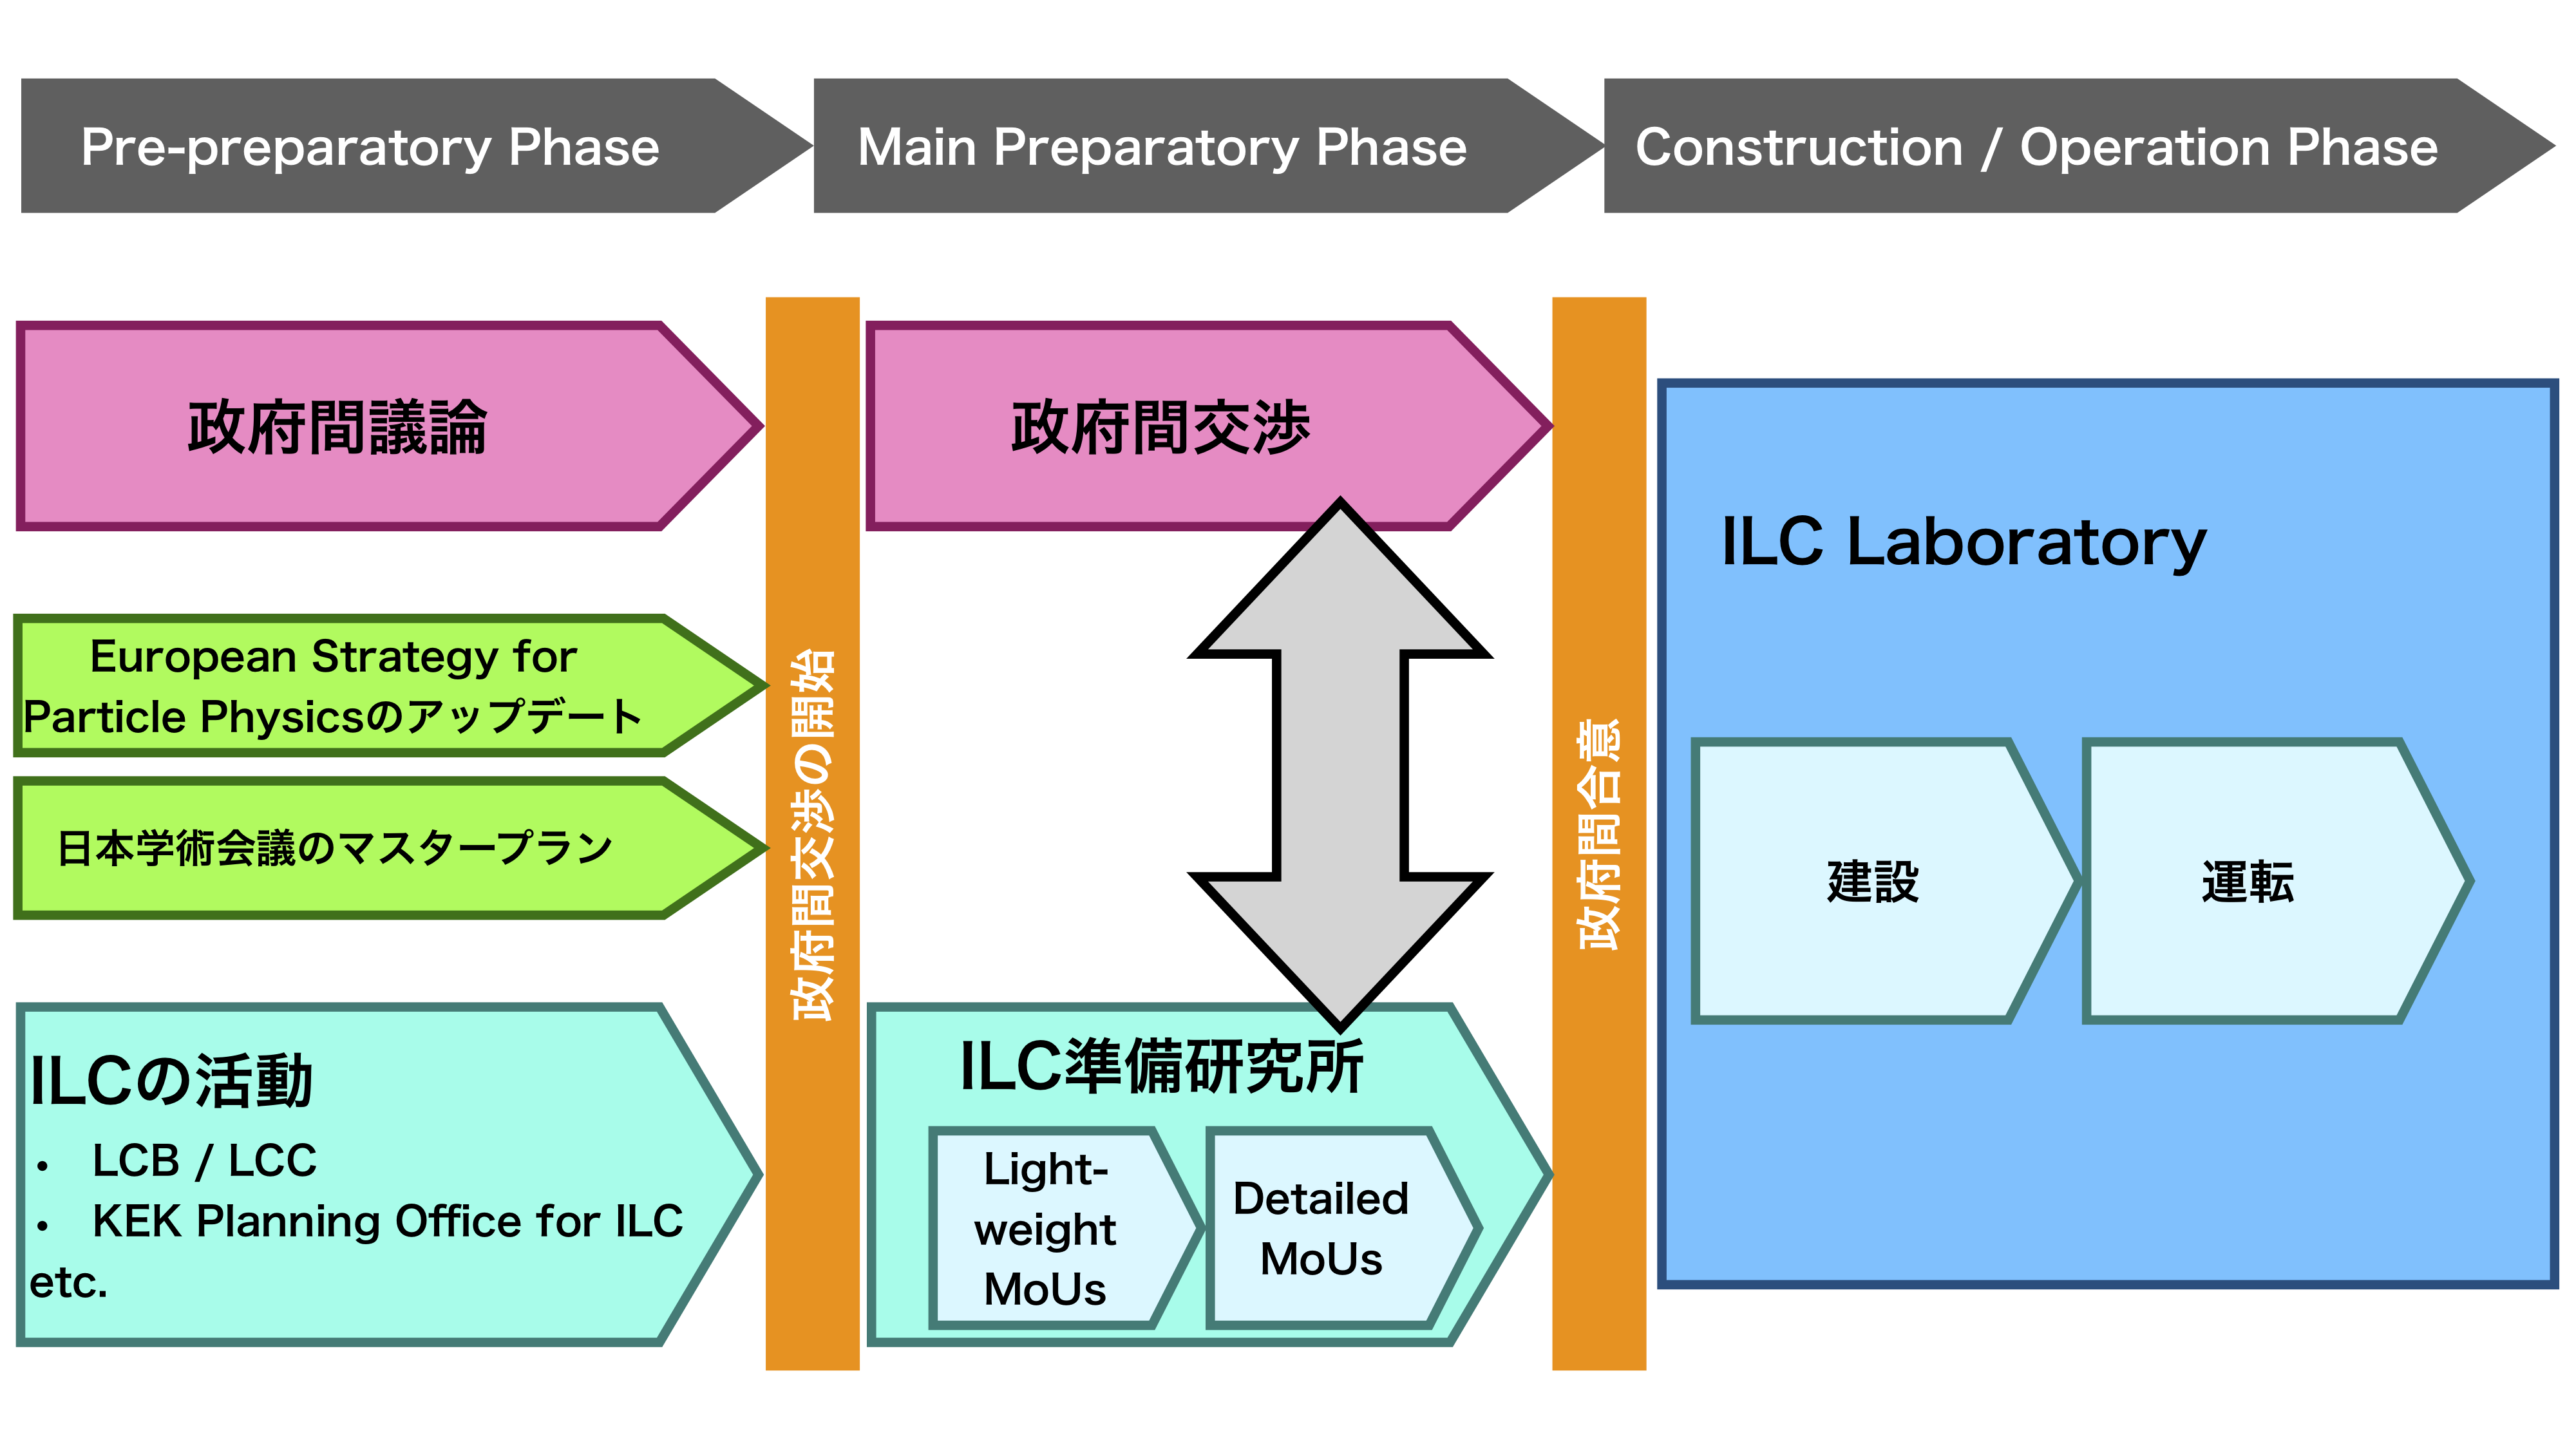
\includegraphics[width=0.85\textwidth]{Figure/1Introduction/3ILCProject.png}
 \caption[ILC計画の今後]
                {ILC計画の今後\cite{RecommendationsonILCProjectImplementation}}
 \label{3ILCProject}
\end{figure}


%%%%%%%%%%%%%%%%%%%%%%%%%%%%%%%%%%%%%%%%%%%%%%%%%%%%%%%%%%%%%%%%%%%%%%%%%%%%%%%%%%%%%%%%%%%%%%%%%%%%%
\section{ILCの物理} \label{Intro:PhysicsofILC}

ヒッグス粒子が2012年に欧州原子核研究機構 (CERN) の大型ハドロン衝突型加速器 (Large Hadron Collider, LHC) で発見されて以降, ヒッグス粒子の性質について, より詳細な調査が行われている。
ヒッグス機構は標準模型の中で電弱相互作用の対称性を破り素粒子に質量を与える役割を担っており, またヒッグス粒子は質量に比例した結合定数を持つという特徴を持っている。
このような性質からヒッグス粒子の振る舞いは標準模型によって詳細に決定され, BSMによって標準模型の素粒子の振る舞いに変化が生じた場合, ヒッグス粒子はその影響を受けると予想されている。
特にヒッグス粒子の結合定数は, そのようなBSMの模型やパラメータの違いによって異なった変化をするため, ヒッグス粒子の結合定数を調べる事によってBSMの探索やその模型識別が可能である。

ILCは, このヒッグス粒子の性質を詳細に調べ, 新物理を発見する為のヒッグスファクトリーとしての役割が期待されている。
LHCが陽子-陽子を衝突させる加速器であるのに対し, ILCは電子-陽電子を衝突させる加速器である。
電子と陽電子は粒子と反粒子の関係となっており, ILCはLHCと比較して目的とする事象に対しエネルギーをより効率的に使うことができる。
更に電子-陽電子衝突の場合は相互作用の関係から, 背景事象が少ないという特徴を持っている。

ILCは電子・陽電子衝突によって, Z粒子とヒッグス粒子を生成する$\it e^+e^- \to Zh$事象の反応断面積が最大となる重心系エネルギー$\sqrt{s}=250\ \mathrm{GeV}$での運転開始 (ILC250) を予定している(図\ref{4eetoZH})。
また, ILCには様々な物理目標を達成する為に多数のアップグレードオプションが存在し, 重心系エネルギーについては主線形加速器を延長, 加速勾配を上昇することで$1\ \mathrm{TeV}$以上への拡張が可能である。\\

\begin{figure}[htbp]
 \centering
 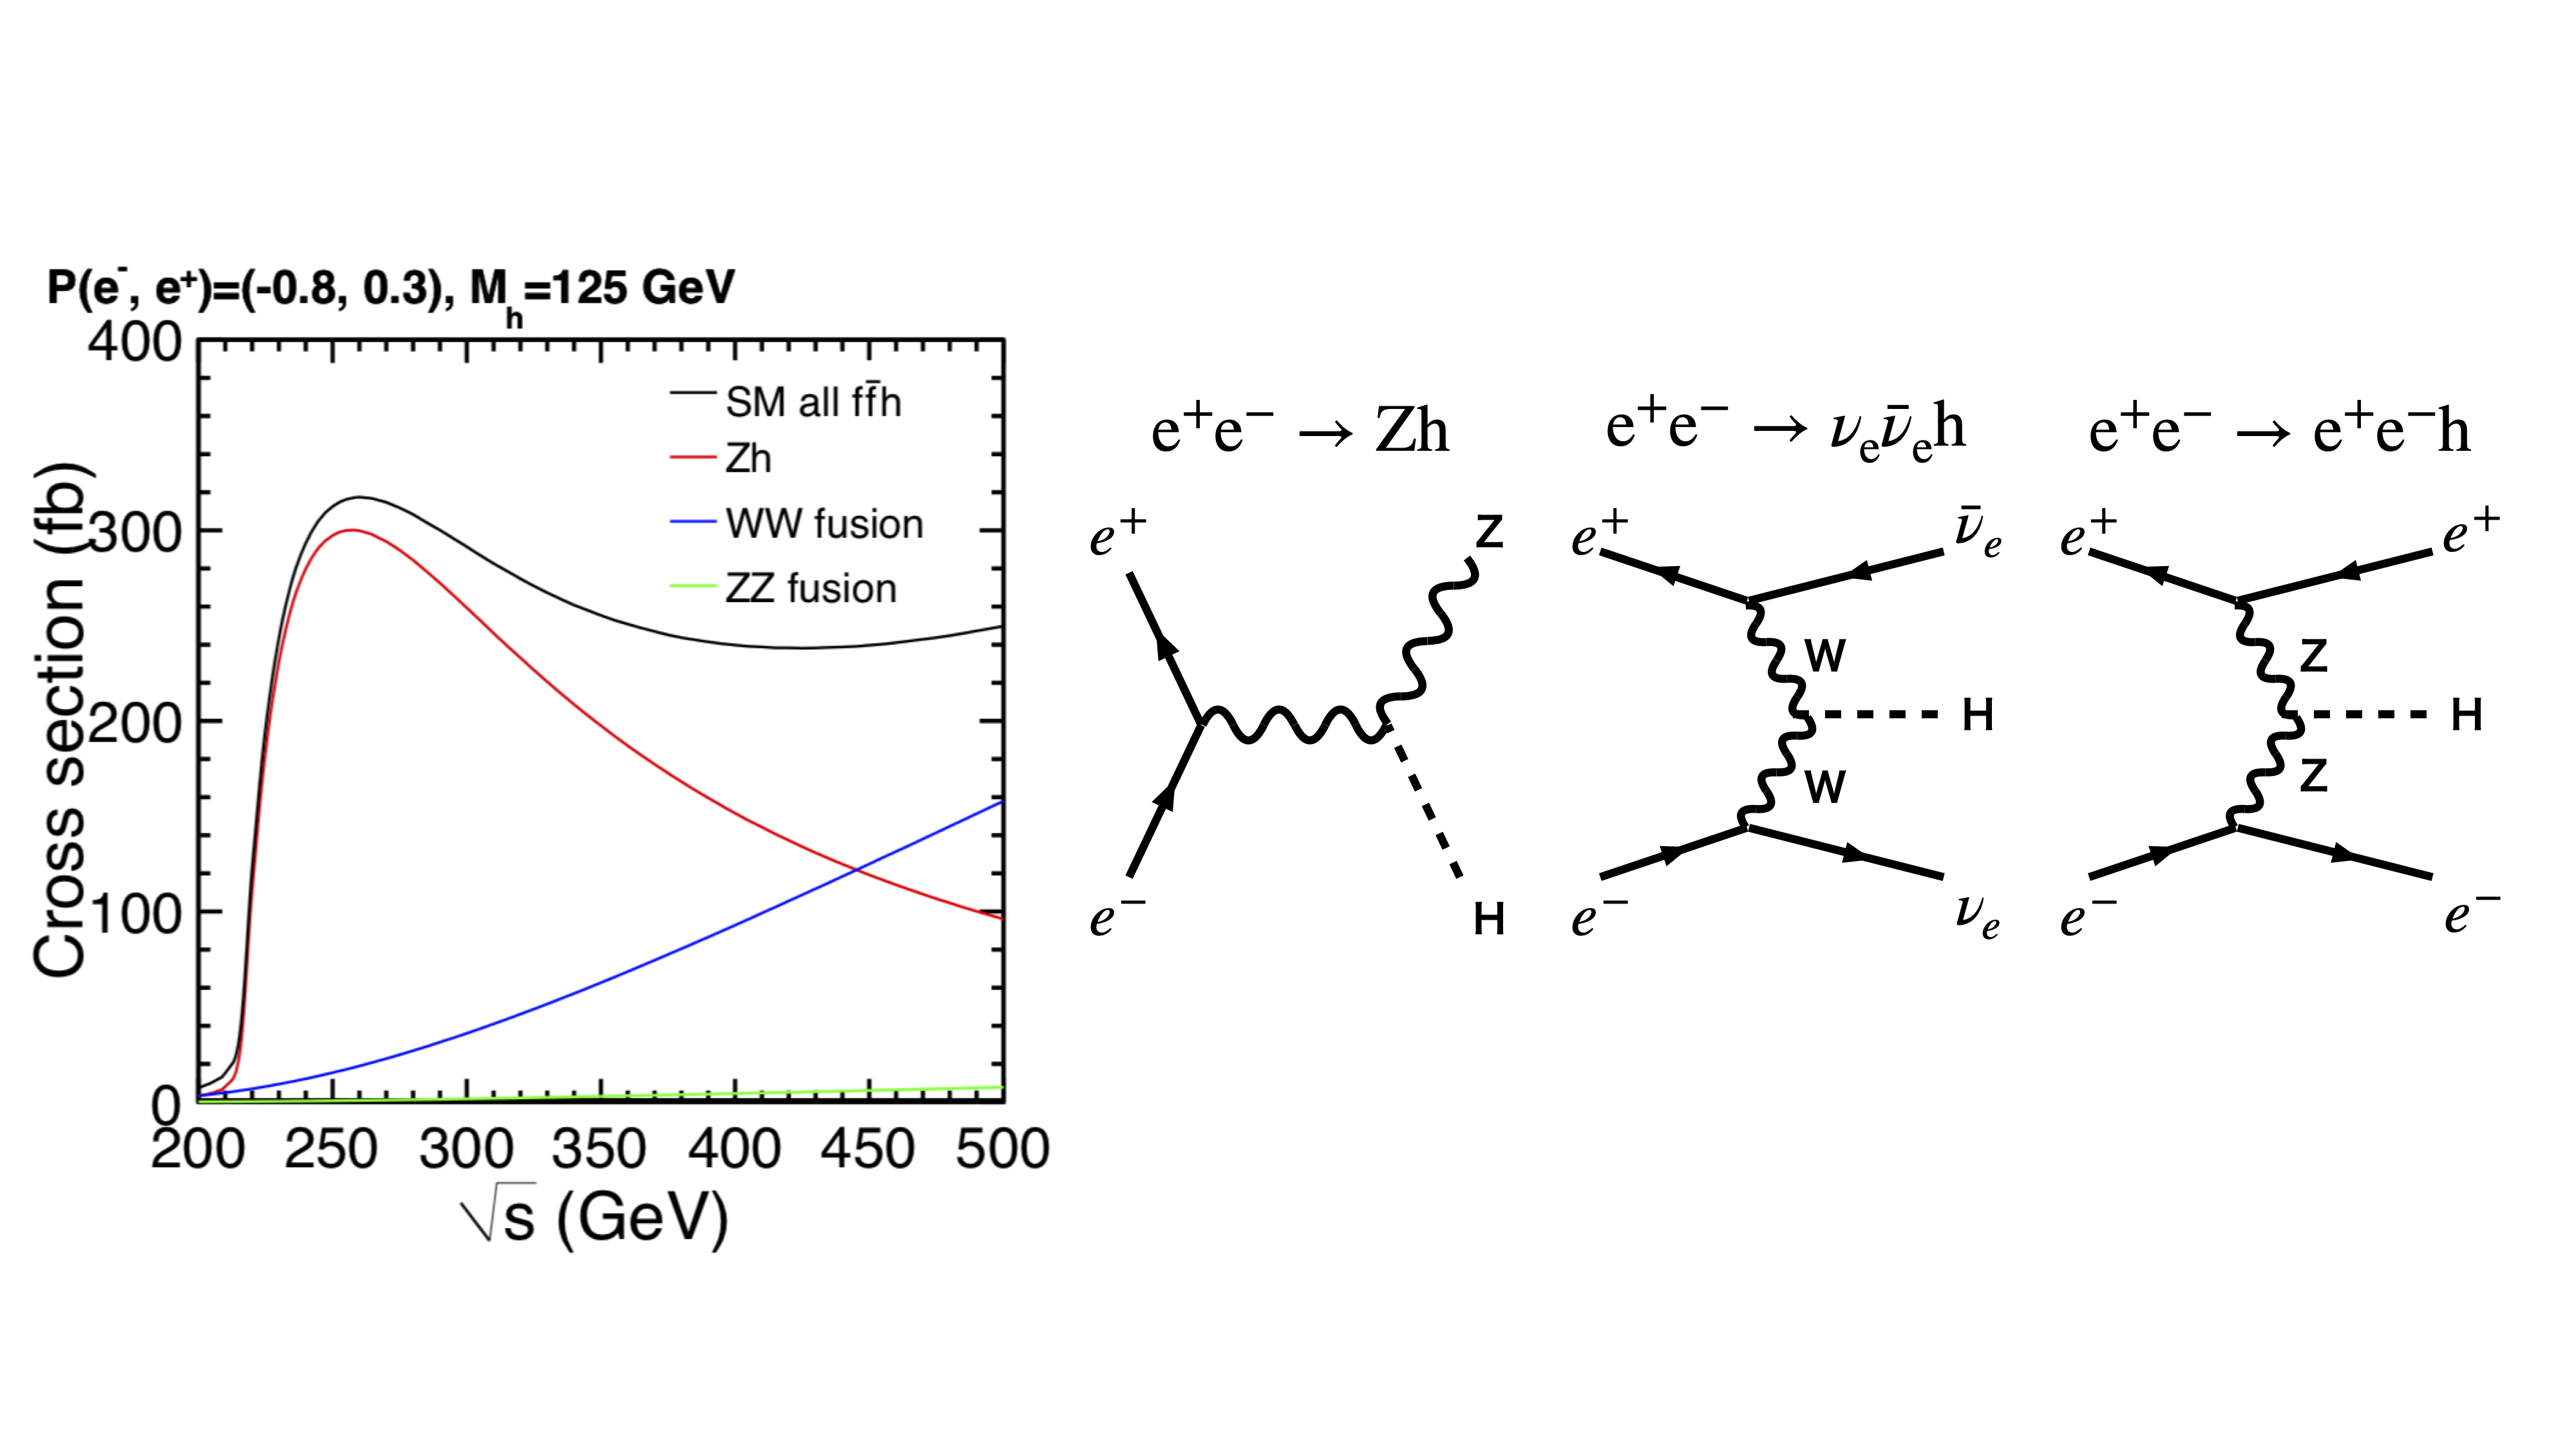
\includegraphics[trim= 0 50 0 50, width=0.9\textwidth, clip]{Figure/1Introduction/4eetoZH.png}
 \caption[重心系エネルギーとヒッグス事象生成断面積の関係]{重心系エネルギーとヒッグス事象生成断面積の関係\cite{ILCTDRVP}。ヒッグス粒子の質量を$125\ \mathrm{GeV}$とした時の$\it e^+e^- \to Zh$事象の生成断面積を赤線でプロットしている。また, WW fusion $\it e^+e^- \to \nu \bar{\nu} h$事象, ZZ fusion $\it e^+e^- \to e^+ e^- h$事象をそれぞれ青線, 緑線で表現している。}
 % The International Linear Collider Technical Design Report - Volume 2: Physics Fig 2.7
 \label{4eetoZH}
\end{figure}

$\it e^+e^- \to Zh$事象はヒッグス粒子の反跳粒子である$\it Z$粒子を再構成することによって, ヒッグス粒子の崩壊モードに寄らずヒッグス粒子を識別・測定できるという点で非常に重要である。
また, 背景事象である$\it e^+e^- \to Z\gamma$事象や$\it e^+e^- \to ZZ$事象に関してもよく理解されており, 電弱相互作用の計算によって不定性を$0.1\ \%$程度に抑えることができる\cite{GlobalProject}。
この反跳粒子を使用した解析では$\it e^+e^- \to Zh$事象の全断面積を得ることができ, 絶対正規化されたヒッグス粒子の結合定数やヒッグス粒子の暗黒物質への崩壊についての測定が可能となる。

ILCではヒッグス粒子の崩壊分岐比について, BR($\it h \to b \bar{b},\ c \bar{c},\ gg,\ WW^*,\ ZZ^*$)の精密測定が期待されている。
特にBR($\it h \to b \bar{b},\ c \bar{c}$)の精密測定は, 第3, 2世代のクォークとヒッグス粒子についての湯川結合を理解する為の手がかりとして非常に重要である。\\

\newpage
これらの重いクォーク対は, それぞれ真空中でクォークの粒子反粒子対を生成・結合しハドロンとなる。
更に, この過程で生成されたクォークも同様にハドロンを形成するため, 初めのクォーク対のそれぞれの進行方向には多数のハドロン粒子が生成されることとなる。
これをジェットといいBR($\it h \to b \bar{b},\ c \bar{c},\ g \bar{g}$)の精密測定では, このジェットの元となったクォークのフレーバーを高精度に同定する必要がある。
このジェットの再構成については, \ref{Intro:SoftERILC:JetReconstruction}項にて説明する。


%%%%%%%%%%%%%%%%%%%%%%%%%%%%%%%%%%%%%%%%%%%%%%%%%%%%%%%%%%%%%%%%%%%%%%%%%%%%%%%%%%%%%%%%%%%%%%%%%%%%%
\section{ILCの検出器 -International Large Detector (ILD)-} \label{Intro:InternationalLargeDetector}

ILCではSilicon Detector (SiD) とInternational Large Detector (ILD) の二つの検出器コンセプトが検討されている。
本研究はILDの検出器シミュレーションデータを用いている為, 本節ではILDについて簡単な解説を行う。
ただし, 本研究の基本的な発想はそのような検出器の違いに寄らず使用することができる。

ILDはヒッグス粒子や電弱相互作用の物理からの要求値を満たすように設計され, また後述するparticle flow algorithm (PFA) (\ref{Intro:SoftERILC:ParticleReconstruction}項) によって最適化されている。
またILDは様々なサブディテクターによって構成され, ビームの衝突点 (図\ref{5-1InternationalLargeDetector}の右下) を包む様に内側から順に, Vertex Detector (VTX), Silicon Internal Tracker (SIT), Time Projection Chamber (TPC), 電磁カロリメータ (ECAL), ハドロンカロリメータ (HCAL), Iron Yoke (Muon) が並んでいる。
また, HCALとIron Yokeの間には超伝導ソレノイドがあり, $3.5 \mathrm{T}$の磁場をかけている。
ILDでは, VTXやSIT, TPCを用いて荷電粒子の飛跡を測定し, ECALによって電子や光子, HCALによってハドロン粒子のエネルギーを測定する。

衝突点の前方, 後方方向には, Forward Tracking Detector (FTD), Luminosity Calorimeter (LumiCAL), LHCAL, Beam Calorimeter (BeamCAL) が並んでいる。
これらのサブディテクターは輝度の測定やビーム状態の監視などを行っている。
それぞれのサブディテクターの詳細については表\ref{ILDSubdetectorParametersBarrel}と表\ref{ILDSubdetectorParametersEndCap}にまとめる。

\begin{figure}[htbp]
 \centering
 \begin{minipage}{1.0\textwidth}
  \centering
   \begin{minipage}{0.48\textwidth}
    \centering
    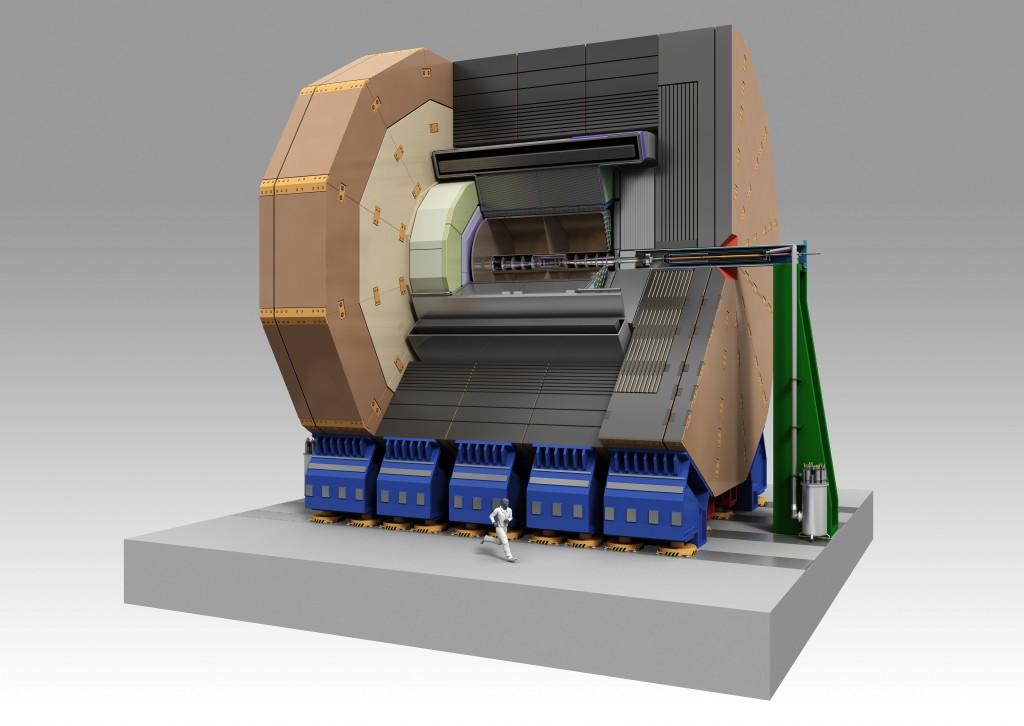
\includegraphics[width=1.0\textwidth, clip]{Figure/1Introduction/5-1InternationalLargeDetector.jpg}
    \subcaption{ILDの全体像\cite{ILCPHOTO}}
   \end{minipage}
   \begin{minipage}{0.48\textwidth}
   \centering
    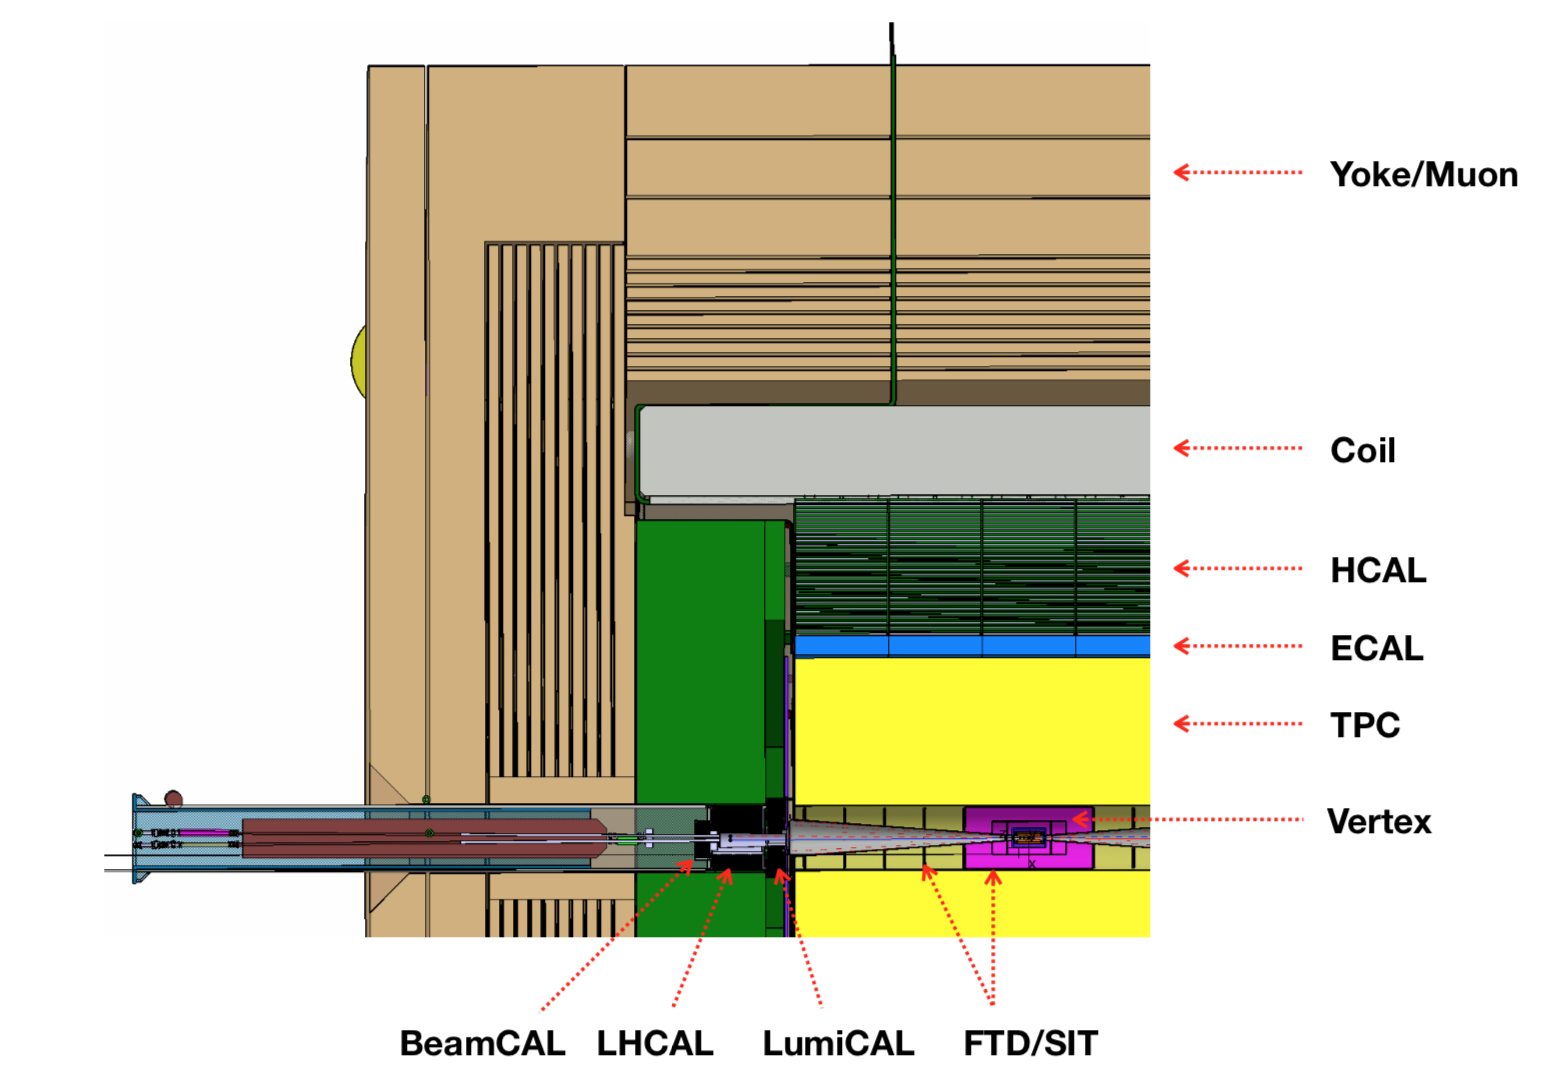
\includegraphics[width=1.0\textwidth, clip]{Figure/1Introduction/5-2InternationalLargeDetector.png}
    % INTERIM DESIGN REPORT Figure 5.1
    \subcaption{ILDの縦断面\cite{InterimDesignReport}}
   \end{minipage}
  \end{minipage}  
  \caption{International Large Detector (ILD) }
  \label{5-1InternationalLargeDetector}
\end{figure}

\begin{table}[htbp]
 \centering
  \small
   \caption[ILDサブディテクターの詳細なパラメータ (バレル)]{ILDサブディテクターの詳細なパラメータ (バレル) \cite{InterimDesignReport}}
   \scalebox{0.9}{
  \begin{tabular*}{1.0\textwidth}{@{\extracolsep{\fill}}l c c c l}\hline
     & $r_{in} \mathrm{[mm]}$ & $r_{out} \mathrm{[mm]}$ & $z_{max} \mathrm{[mm]}$ & 要素技術\\ \hline \hline
    VTX & 16 & 60 & 125 & シリコンピクセルセンサー\\
    SIT & 153 & 303 & 644 & シリコンピクセルセンサー\\
    TPC & 329 & 1770 & 2350 & マイクロパターンガス検出器\\
    SET & 1773 & 1776 & 2300 & シリコンストリップセンサー\\ \hline
    ECAL & 1805 & 2028 & 2350 & 吸収層 : タングステン\\
    &&&& センサー : シリコン/シンチレーター\\
    HCAL & 2058 & 3345 & 2350 & 吸収層 : スチール\\
    &&&& センサー : シンチレーター/RPCガス\\ \hline
    Coil & 3425 & 4175 & 3872\\
    Muon & 4450 & 7755 & 4047 & センサー : シンチレーター\\ \hline
  \end{tabular*}
  }
  \label{ILDSubdetectorParametersBarrel}
\end{table}

\begin{table}[htbp]
 \centering
 \small
\caption[ILDサブディテクターの詳細なパラメータ (エンドキャップ)]{ILDサブディテクターの詳細なパラメータ (エンドキャップ) \cite{InterimDesignReport}}
 \scalebox{0.9}{
  \begin{tabular*}{1.0\textwidth}{@{\extracolsep{\fill}}l c c c c l}\hline
     & $z_{min} \mathrm{[mm]}$ & $z_{max} \mathrm{[mm]}$ & $r_{in} \mathrm{[mm]}$ & $r_{out} \mathrm{[mm]}$ & 要素技術\\ \hline \hline
    FTD & 220 & 371 & & 153 & シリコンピクセルセンサー\\
            & 645 & 2212 & & 300 & シリコンストリップセンサー\\ \hline
    ECAL & 2411 & 2635 & 250 & 2096 & 吸収層 : タングステン\\
    &&&&& センサー : シリコン/シンチレーター\\
    HCAL & 2650 & 3937 & 350 & 3226 & 吸収層 : スチール\\
    &&&&& センサー : シンチレーター/RPCガス\\
    Muon & 4072 & 6712 & 350 & 7716 & センサー : シンチレーター\\ \hline
    BeamCAL & 3115 & 3315 & 18 & 140 & 吸収層 : タングステン\\
    &&&&& GaAs読み出し \\
    LumiCAL & 2412 & 2541 & 84 & 194 & 吸収層 : タングステン\\
    &&&&& センサー : シリコン\\
    LHCAL & 2680 & 3160 & 130 & 315 &吸収層 : タングステン\\ \hline
  \end{tabular*}
  }
  \label{ILDSubdetectorParametersEndCap}
\end{table}

%%%%%%%%%%%%%%%%%%%%%%%%%%%%%%%%%%%%%%%%%%%%%%%%%%%%%%%%%%%%%%%%%%%%%%%%%%%%%%%%%%%%%%%%%%%%%%%%%%%%%
\section{ILCのソフトウェアと事象再構成} \label{Intro:SoftwareandEventReconstructionofILC}

ここではILCで使用されるソフトウェアと事象再構成について述べる。
事象再構成とは, 加速器実験によって得られるデータから飛跡やジェットなどの物理情報を再構成するアルゴリズムである。
そのような再構成は電子-陽電子の衝突毎に行われ, この衝突一回分の事を事象という。

ILCのソフトウェアはiLCSoft\cite{iLCSoft}と呼ばれるソフトウェアエコシステムにまとめられている。

ILCにおける事象再構成は, 飛跡再構成やPFAといった粒子の再構成 (\ref{Intro:SoftERILC:ParticleReconstruction}項) と, 更にそれらによって再構成された粒子を用いたジェットの再構成 (\ref{Intro:SoftERILC:JetReconstruction}項) に区分できる。
ジェットの再構成は崩壊点検出, ジェットクラスタリング, フレーバータギングという行程で行われ, ジェット再構成アルゴリズムとしてiLCSoft内のLCFIPlus\cite{LCFIPlus, LCFIPlusPaper}というソフトウェアが使用されている。


%%%%%%%%%%%%%%%%%%%%%%%%%%%%%%%%%%%%%%%%%%%%%%%%%%%%%%%%%%%%%%%%%%%%%%%%
\subsection{ソフトウェア} \label{Intro:SoftERILC:Software}

ILCは実際の実験データをまだ取得できないため, 本研究で使用するデータは全てシミュレーションデータである。
シミュレーションデータは標準模型とBSMの模型を用いて, モンテカルロ (Monte Carlo, MC) 法によって生成されている。
それらのシミュレーションデータはLCIOと呼ばれる階層型のEvent Data Model (EDM) によって管理されている。
LCIOでは, MC情報から事象の生データ, デジタル化, 解析や後述する再構成に至るまでが紐づけられており, 階層的に取り扱うことができる。

ILCのソフトウェアは二つの検出器コンセプト (ILD, SiD) で概ね共通しており, 前述したように現在はiLCSoftというソフトウェアエコシステムによって統括されている。
提供されているAPIの言語はC++・java・Fortranである。

それらソフトウェアモジュールはMarlin\cite{Marlinpaper}というC++アプリケーションフレームワークによって運用されており, プロセッサーと呼ばれるモジュールを作成・組み込むことにより, 様々な再構成・解析アルゴリズムを簡単に別のモジュールへ置き換えることができる。
また, データの入出力はLCIO, ROOTフォーマットによって行われる。

\newpage
%%%%%%%%%%%%%%%%%%%%%%%%%%%%%%%%%%%%%%%%%%%%%%%%%%%%%%%%%%%%%%%%%%%%%%%%
\subsection{飛跡の再構成} \label{Intro:SoftERILC:ParticleReconstruction}

飛跡の再構成は, シミュレーションされた検出器のデータから, 粒子 (飛跡) を再構成する飛跡再構成と, そのようにして得られた個々の飛跡検出器 (VTX, SIT, TPCなど) の粒子についての情報を繋ぎ合わせ, より高精度の粒子情報を提供するPFAという手順によって行われる。\\

飛跡再構成\\

飛跡再構成では, まず荷電粒子の飛跡をパターン認識を用いて再構成し, 次にそれらの飛跡について運動学的な物理量をフィッティングによって抽出している。
LCIOにおいて飛跡は飛跡の曲率$\rm \Omega$, インパクトパラメータ$\rm d_0$, $\rm z_0$, 方向パラメータ$\rm \phi$, $\rm \tan{\lambda}$のperigee track parameterizationによって保持されている。
ILDにおいて異なるサブディテクターの飛跡再構成は異なるアルゴリズムが使用されている。\\

Particle Flow Algorithm\\

飛跡再構成によって運動学的な物理量を得られるのは荷電粒子のみである。
中性粒子はVXDやTPCに飛跡を残さない為, カロリメータ (ECAL, HCAL) を用いた再構成が必要となる。
このように粒子の性質によって, 再構成を行うべき最適なサブディテクターは異なっている。
ILCではparticle flow algorithm (PFA) を用いた高い粒子識別を目指している。
PFAにおいて荷電粒子は飛跡検出器によって測定され, 光子や中性ハドロンはそれぞれECALやHCALによって再構成されている。
PFAではジェット中の個々の粒子を分離する事によって, ジェットエネルギー分解能の大幅な向上が期待されており, その実現には高精細なカロリメータと高精度な飛跡検出器が必要となる。

iLCSoftではPandoraPFAというアルゴリズムが使用されている。
このアルゴリズムでは, まずカロリメータのヒットをクラスター化し, それらクラスターとトラッキング情報を関連づけ荷電粒子と中性粒子の分離を行っている。
出力はPandoraPFOと呼ばれる再構成された粒子のオブジェクトであり, これは以降の解析や更なる再構成に使用可能である。\\

以上が飛跡の再構成である。
飛跡の再構成では, 検出器で得られた情報から粒子を再構成するまでを行なっている。
実際には注目すべき物理事象は前述したジェットのような特徴的なシグネチャを残す為, 次項のジェットの再構成による更なる解析が必要である。


%%%%%%%%%%%%%%%%%%%%%%%%%%%%%%%%%%%%%%%%%%%%%%%%%%%%%%%%%%%%%%%%%%%%%%%%
\subsection{ジェットの再構成} \label{Intro:SoftERILC:JetReconstruction}

事象中に生じたクォークは\ref{Intro:PhysicsofILC}節で述べたようにジェットを形成する。
ジェットには多数の粒子 (飛跡) が含まれ, それら多数の粒子の親となる粒子が崩壊した点を崩壊点 (Vertex) という。
特に, ハドロンのような準安定な親粒子の崩壊点の事をsecondary vertexといい, 電子-陽電子の衝突点をprimary vertexという (図\ref{6ReconstructedVertex})。
ジェットの再構成では, まずこの崩壊点を崩壊点検出アルゴリズムを用いて探索し, 得られた崩壊点を用いてジェット中の粒子を分離するジェットクラスタリングが行われる。
最後に, ジェット中の飛跡や崩壊点から親粒子のクォーク・フレーバーを識別するフレーバータギングが行われる。

\begin{figure}[htbp]
 \centering
 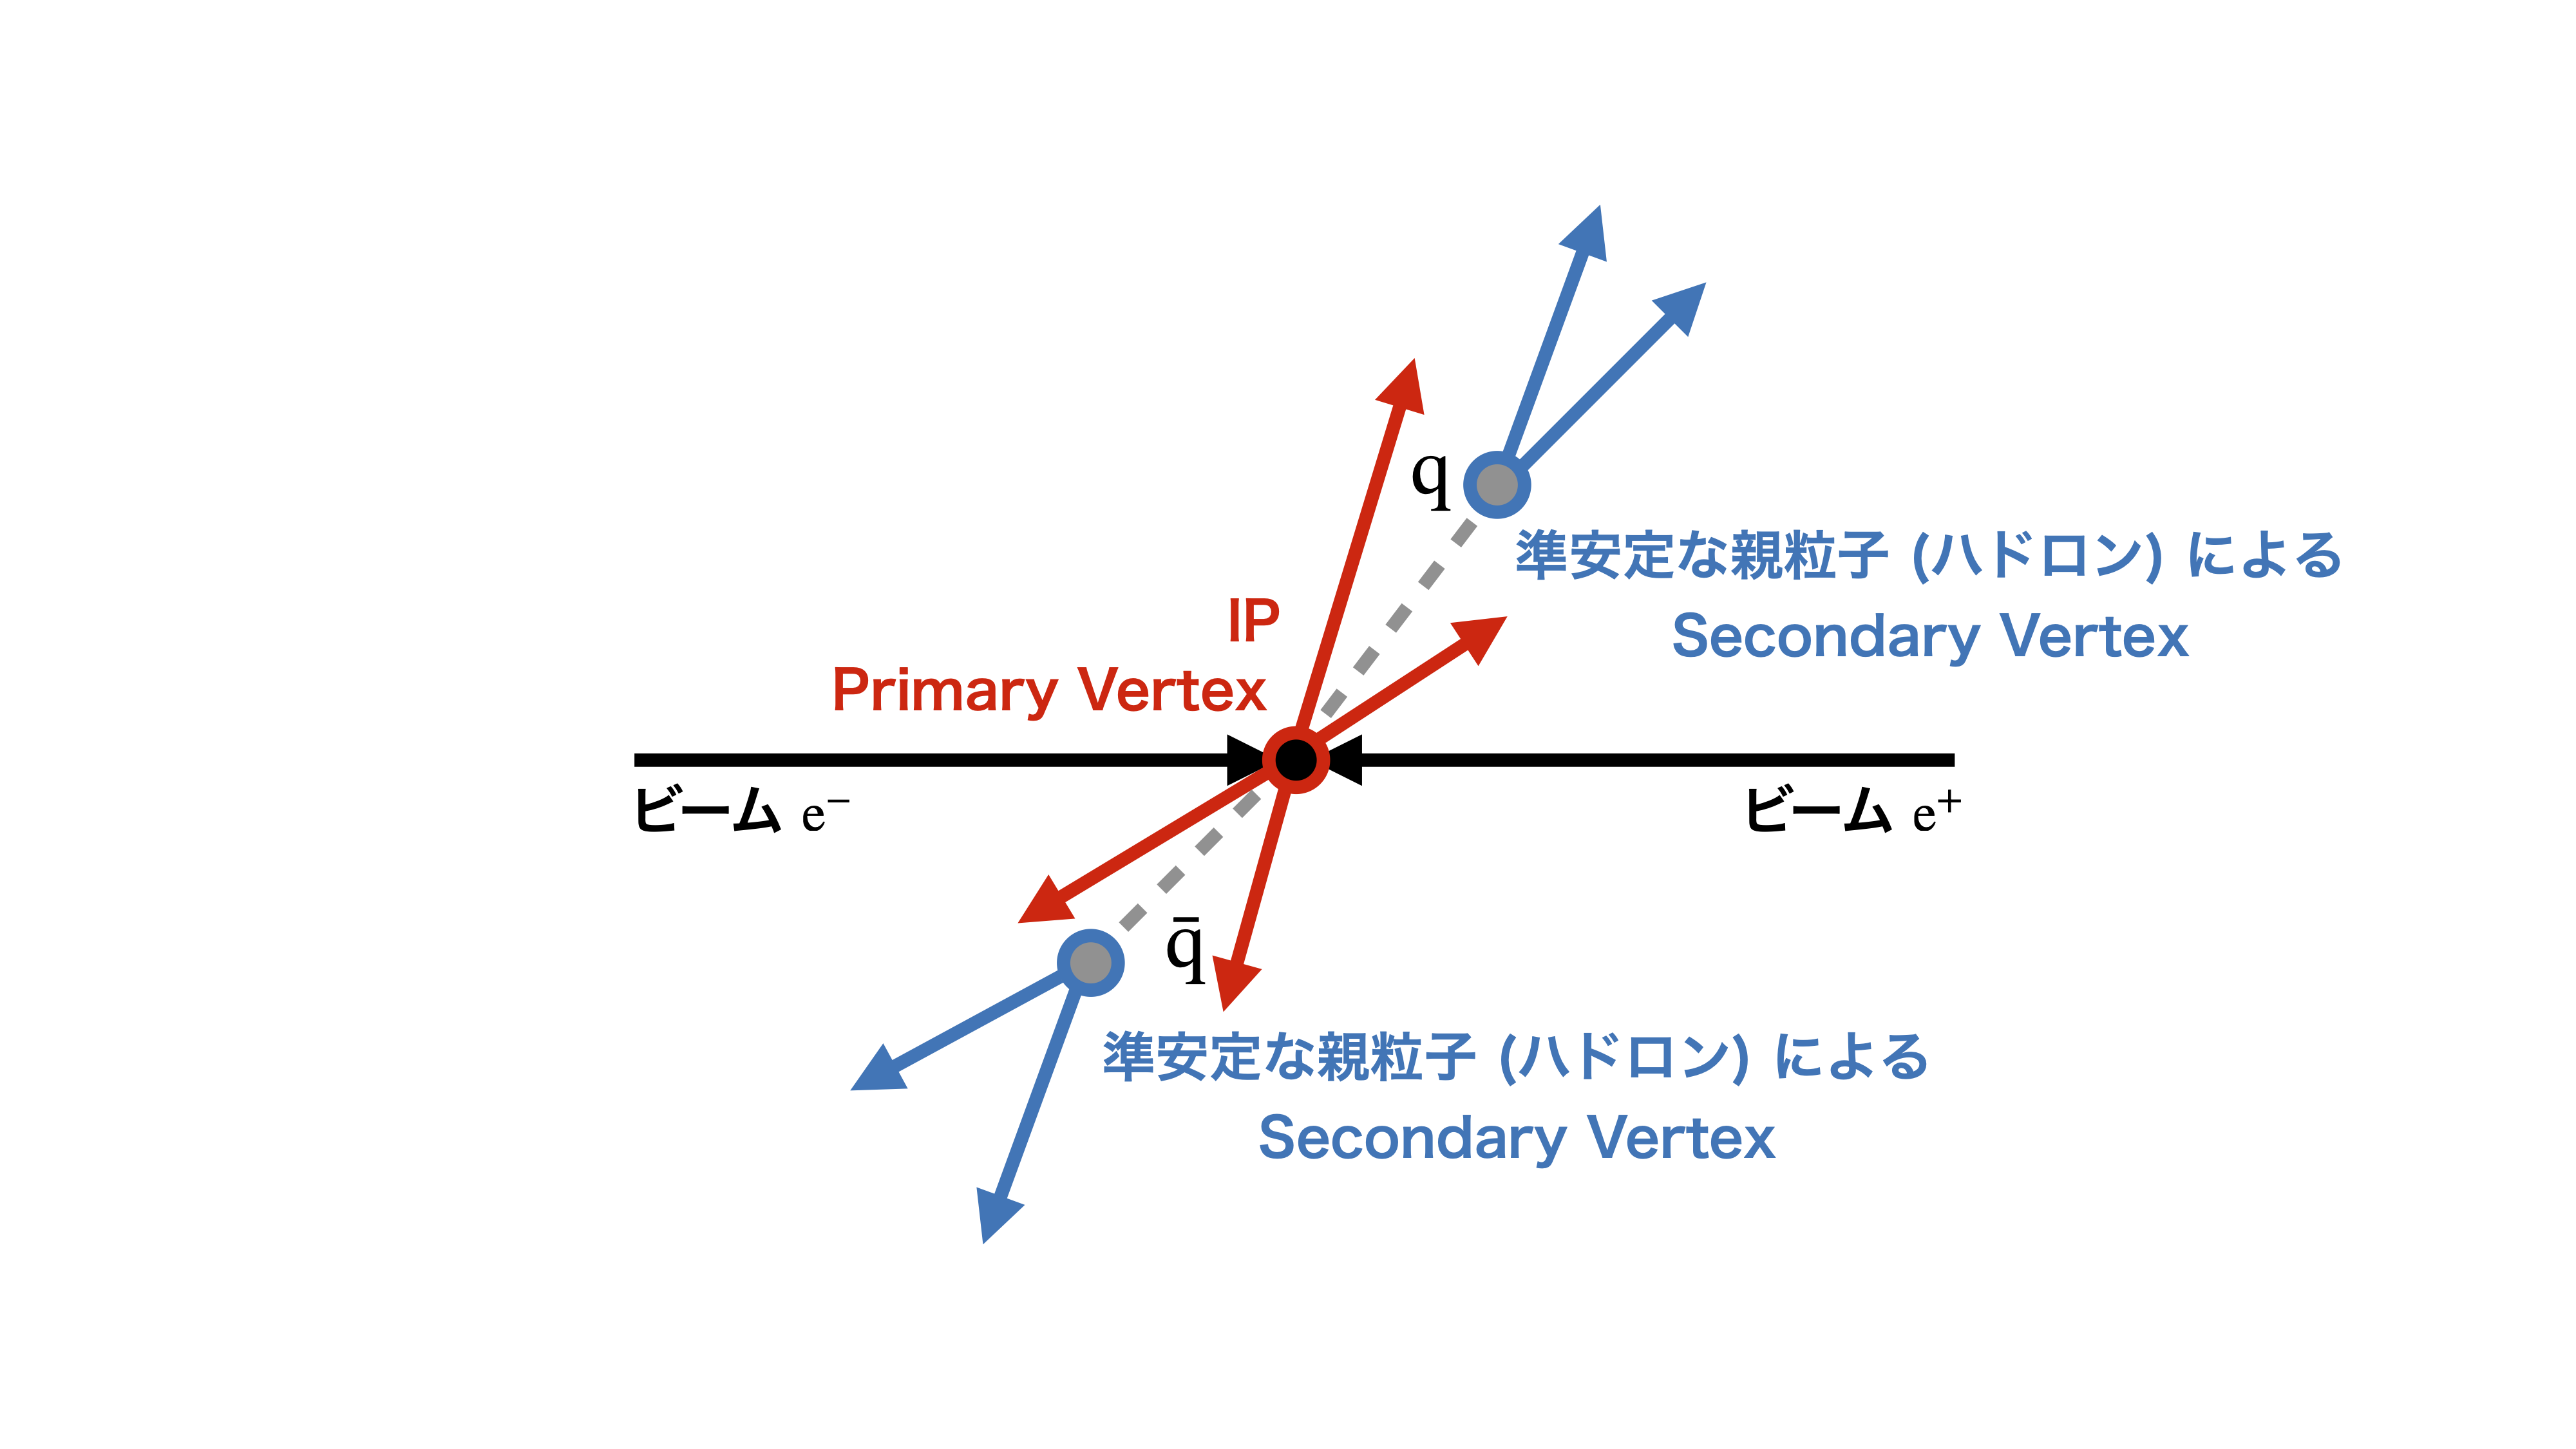
\includegraphics[trim = 0 100 0 100, width=1.0\textwidth, clip]{Figure/1Introduction/6ReconstructedVertex.png}
 \caption[primary vertexとsecondary vertexの図示]{primary vertexとsecondary vertexの図示。左右から電子・陽電子ビームが入射され, 図中央で衝突したと仮定している。灰色の破線は準安定なハドロンを表現しており, 赤線の飛跡と共にIP (primary vertex) から生じている。ハドロンは更に図右上と左下で崩壊し, secondary vertexを残す。青線はこのsecondary vertex由来の飛跡である。}
 \label{6ReconstructedVertex}
\end{figure}

崩壊点検出では, 二本以上の飛跡について交点を求めるフィッティングを用いている。
この時, フィッティングの健全性は$\chi^2$値によって把握している。

まずprimary vertexの再構成をTear-Down法によって行う。
具体的には予想されるビームスポットと事象中の全飛跡についてフィッティングを行い, $\chi^2$値が一定以下になるまで$\chi^2$値への寄与の大きい飛跡を一本ずつ取り除いていく。
残った飛跡をprimary vertex由来であると判定し, 以降の再構成に用いる。

次にsecondary vertexの再構成をBuild-Up法によって行う。
ここでは, primary vertexに含まれていない飛跡について, 二本の飛跡 (飛跡対) の全ての組み合わせを作りフィッティングを行う。
そのようにして得られた$\chi^2$値と運動量の方向, 不変質量などをカットベースに判定し, secondary vertexの候補を選別する。
更に, この飛跡対に対して飛跡を加えていくことでsecondary vertexを再構成している。

崩壊点検出で得られた崩壊点を用いて, ジェットクラスタリングが行われる。
ジェットクラスタリングでは崩壊点の情報を使用して中性粒子の飛跡を含めた全ての飛跡についてクラスタリングを行う。
LCFIPlusではこのジェットクラスタリングの前に, 重いハドロン粒子のセミレプトニック崩壊によって生じた孤立レプトンをエネルギーやインパクトパラメータを用いて探索している。
次に得られた孤立レプトンとsecondary vertexの組み合わせを行う。
孤立レプトンについては運動量方向を, secondary vertexについてはprimary vertexからの角度を用いそれらの開き角が一定の閾値以下であるかによって評価している。
これらの手順により再構成された孤立レプトンや崩壊点はジェットクラスタリングのコアとして使用される。
ジェットクラスタリングはDurhamアルゴリズム\cite{Durhampaper}を用いており, 粒子の運動量方向とジェットの開き角, 修正Durham距離に基づいてジェットの再構成を行っている。

LCFIPlusではジェットのフレーバーをより精度よく同定するためにjet vertex refinerアルゴリズムが使用されている。
jet vertex refinerはシングルトラック崩壊点検出と崩壊点コンバイナの二つのステップで行われる。
シングルトラック崩壊点検出では崩壊点を一つしか含まないジェットについて, 飛跡を一本だけ含む疑似崩壊点を探索するアルゴリズムである。
崩壊点コンバイナは二つ以上の崩壊点を含むジェットについて崩壊点の個数を最大二つに結合させるアルゴリズムである。
ジェット中の崩壊点について更に一つに纏められる場合は新たな崩壊点への置き換えを行う。\\

クラスター化されたジェットについてフレーバー識別が行われる。
フレーバータギングではBoosted Decision Trees (BDTs) を用いて親粒子のフレーバーを識別している。
BDTsはROOTのTMVAパッケージを使用し, ボトム・フレーバーのジェット, チャーム・フレーバーのジェット, アップ, ダウン, ストレンジ・フレーバーのジェットの三つにクラスで分類している。
入力変数はジェット内の崩壊点や飛跡などの構成要素によって作成され, ジェットのエネルギーに依存する様な変数については規格化を行っている。\\

以上がジェットの再構成である。
様々な物理解析において, ジェットの個数やそのフレーバーの識別は信号事象と背景事象の弁別や物理解析などに使用されている。
したがって, ジェットの再構成の性能向上はあらゆる物理解析の性能向上と直結していると言える。


%%%%%%%%%%%%%%%%%%%%%%%%%%%%%%%%%%%%%%%%%%%%%%%%%%%%%%%%%%%%%%%%%%%%%%%%%%%%%%%%%%%%%%%%%%%%%%%%%%%%%
\section{本研究の目的} \label{Intro:Purpose}

本研究の目的は, 深層学習を使用して\ref{Intro:SoftERILC:JetReconstruction}項で紹介した崩壊点検出を開発・改善することである。
ILCでは現在LCFIPlus内の崩壊点検出が使用されているが, primary vertexやsecondary vertexの選別に人が定めた閾値が多く含まれており, それら閾値に基づいた選定を行っている。\footnote{この様な手法をカットベースという。}
このような人が定めた閾値は最適ではなく, 何らかの情報を欠損してしまっている可能性がある。
本研究では深層学習を用いたパターン認識の技術から新しい崩壊点検出アルゴリズムを提案し, より柔軟な識別を行うことを目標とする。

また, この研究は深層学習を用いて事象再構成を改善するプロジェクトの一つであり, 最終的には概念図\ref{7JetReconstructionwithDeepLearning}に示すように, 全ての事象再構成アルゴリズムを深層学習やその他の機械学習技術に置き換えることを目指している。
これまでILCの事象再構成では殆ど深層学習は使われておらず, 特に崩壊点検出に関しては前例のない試みである。

\begin{figure}[htbp]
 \centering
 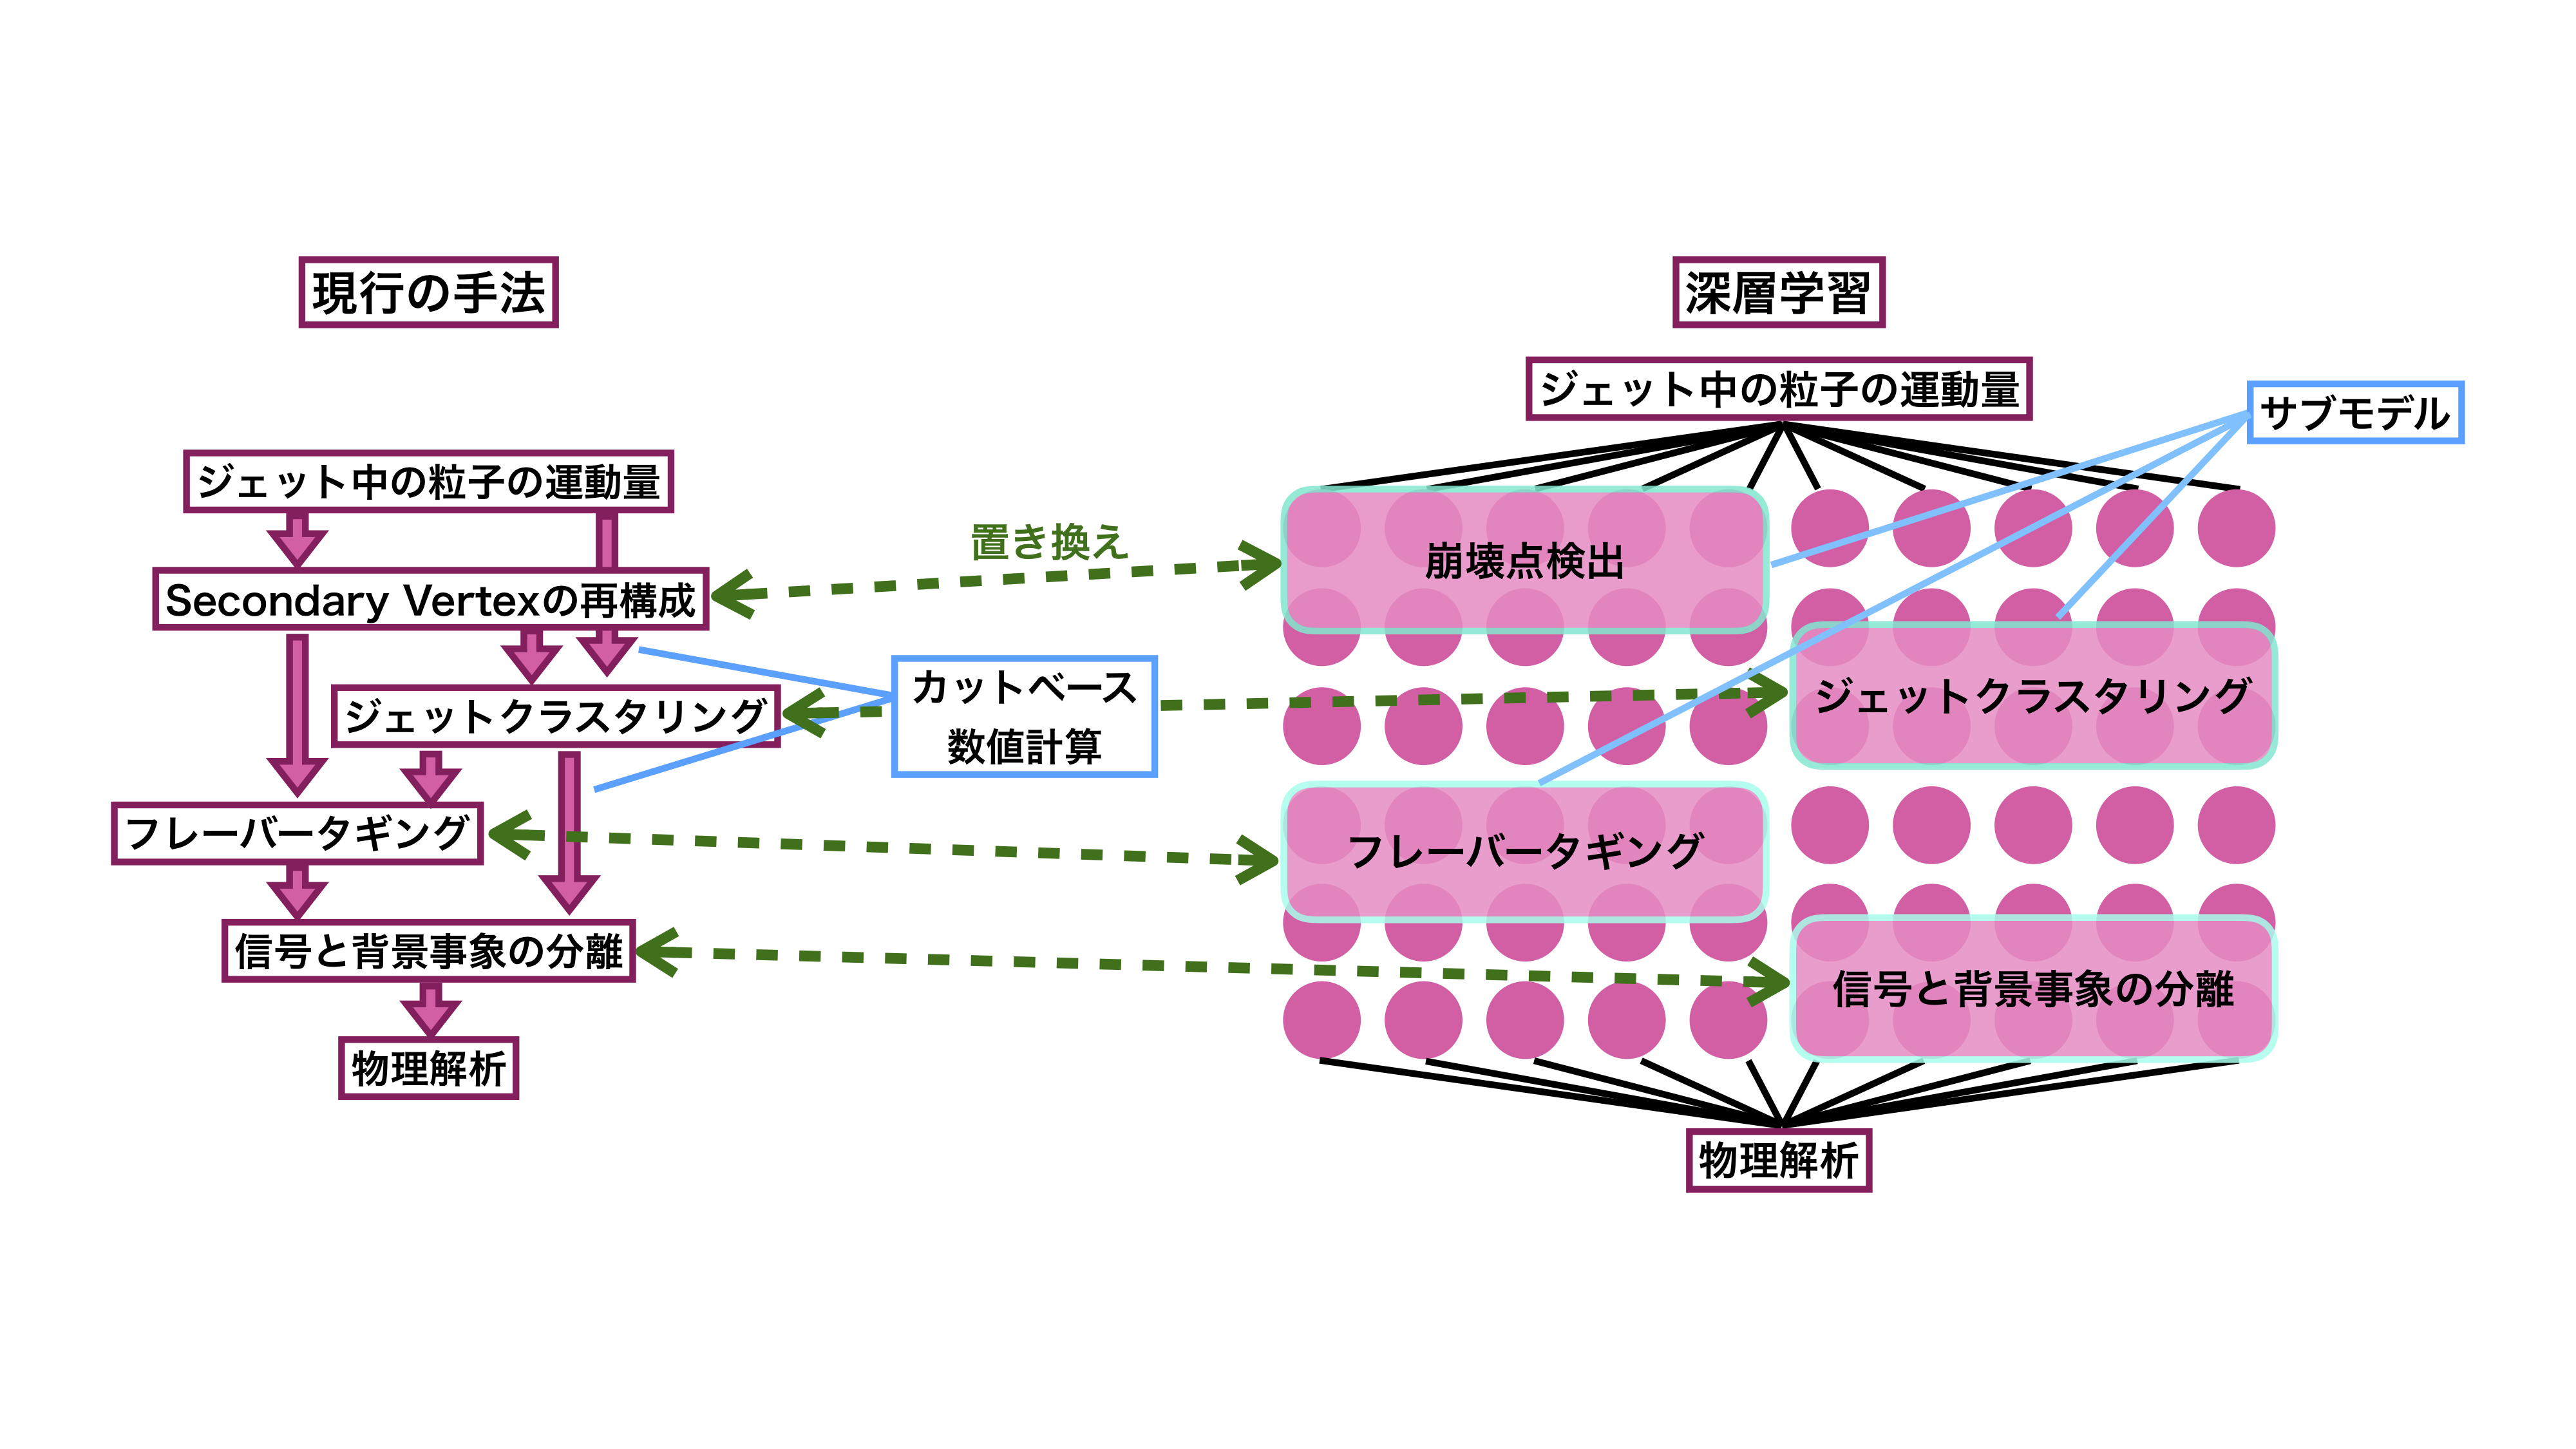
\includegraphics[trim = 0 100 0 50, width=1.0\textwidth, clip]{Figure/1Introduction/7JetReconstructionwithDeepLearning.png}
 \caption[深層学習によるジェットの再構成]{深層学習によるジェットの再構成。図左は現行の手法, 図右は目標としている深層学習を用いた再構成手法の概念図である。現行の手法では多くの場合, 数値計算やそこから得られる変数に閾値を課してカットベースの評価が行われている。現在は深層学習への置き換えの第一段階として, それぞれの役割に特化したサブモデルと入れ替えを行い性能の改善を図っている。}
 \label{7JetReconstructionwithDeepLearning}
\end{figure}

したがって, 本研究のソフトウェア開発としての目的は, 本アルゴリズムを通して次世代のLCFIPlusへの深層学習実装モデルを示す事である。
ここでは, 深層学習の実装・構築からiLCSoftへの導入を行い, ILC研究における深層学習導入の先駆けとなることを目指す。


%%%%%%%%%%%%%%%%%%%%%%%%%%%%%%%%%%%%%%%%%%%%%%%%%%%%%%%%%%%%%%%%%%%%%%%%%%%%%%%%%%%%%%%%%%%%%%%%%%%%%
\section{本論文の流れ} \label{Intro:Flow}

本章と\ref{chap:DeepLearning}章は本論文の導入である。

\ref{chap:DeepLearning}章では本論文の核となる技術である深層学習について解説を行う。
ここでは, 本研究を理解する為に必要な技術領域や背景理論について簡潔な導入を行い, \ref{chap:Networks}章以降では, この\ref{chap:DeepLearning}章の内容を前提とした議論を行う。
ただし深層学習に関しての種々のテクニックについては経験則によるものが多いため, 本研究で使用したものについては\ref{chap:DeepLearning}章では説明せず, \ref{chap:Networks}章で述べる。
また, 具体的な実装に関しても同様に\ref{chap:DeepLearning}章では記載せず, 付録\ref{sec:Code}にまとめる事とする。\\

\ref{chap:Networks}章と\ref{chap:VertexFinderwithDL}章, \ref{chap:Comparison}章は本論文の本題である。
\ref{chap:Networks}章では本研究で使用するデータと作成した深層学習のネットワークについて, その構造の解説や評価を行う。
また, 深層学習を使用した崩壊点検出についての発想や計算環境に関しても\ref{chap:Networks}章で述べる。

\ref{chap:VertexFinderwithDL}章では\ref{chap:Networks}章で作成したネットワークを用いた崩壊点検出について, アルゴリズムや各種最適化, 簡単な評価を行う。

\ref{chap:Comparison}章ではその様にして得られた崩壊点検出と, LCFIPlusで使用されている現行の崩壊点検出との比較について述べる。\\

\ref{chap:Conclusion}章は本論文の結論である。
ここでは, 本研究をまとめると共に今後の展望について述べる。

















